\section{MQTT Publisher branch}
\label{sec:publisher_branch}
In the first branch of the flow, on intervals of five seconds, an MQTT publisher publishes a message onto the topic "challenge3/id\_generator". In this section we will see in a detailed way the workflow of this part.
\begin{figure}[H]
    \centering
    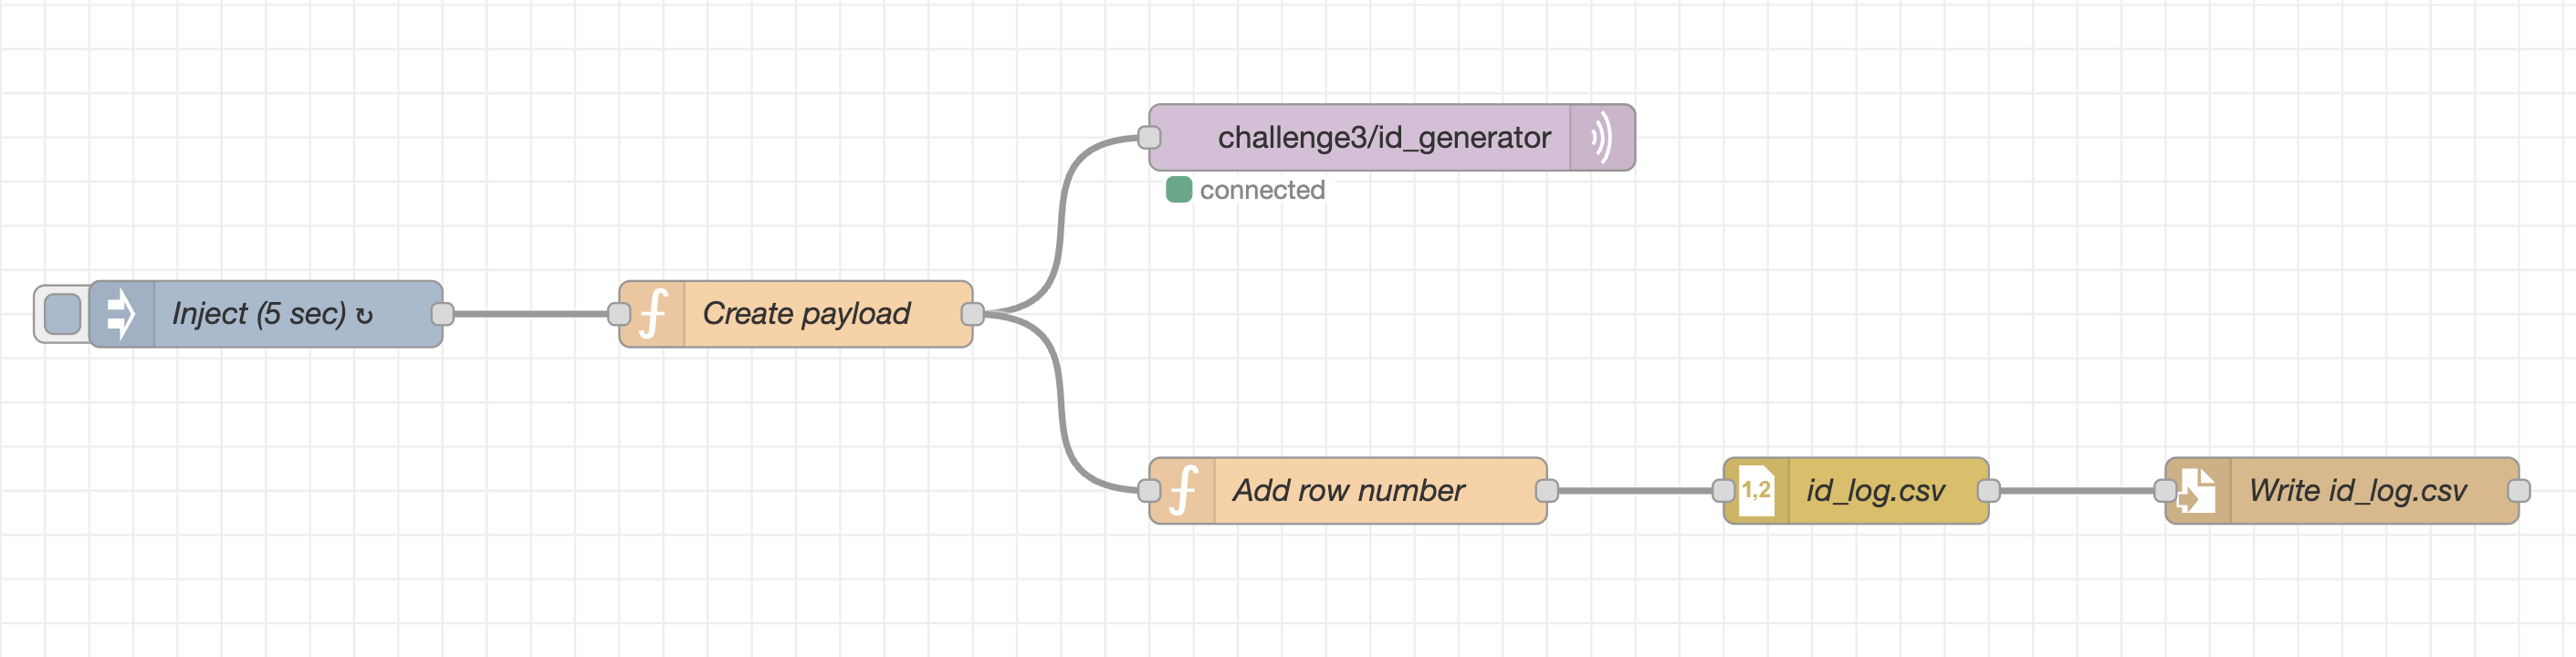
\includegraphics[width=\linewidth, height=0.5\textheight, keepaspectratio]{mqtt_publisher_branch.png}
    \caption{MQTT Publisher branch of the flow}
\end{figure}

\subsection{Inject (5 sec)}
This is the first node and the entry point for the whole system. It starts the process on a deploy and injects a new message every 5 seconds.

\subsection{Create payload}
This is a function node and its purpose is to generate the payload of messages that will be forwarded to the MQTT publisher. \\
The payload is composed by two fields:
\begin{itemize}
\item ID: this field is the Id of the message and is a random integer in the range of 0-30000.
\item TIMESTAMP: this field represents the exact time the message was created.
The code of the function node is reported here.
\begin{minted}{javascript}
let initializationCompleted = flow.get("initializationCompleted") || false;
if (!initializationCompleted) {
    return null;    
}
var id = Math.floor(Math.random() * 30000);
var timestamp = Math.floor(Date.now() / 1000);
msg.payload = {
    id: id,
    timestamp: timestamp
};
return msg;
\end{minted}
\end{itemize}

\subsection{challenge3/id\_generator}
This is the MQTT node that publishes the messages to the local MQTT broker running on port 1884. Messages are published to the topic "challenge3/id\_generator", in this way the subscriber used in the second part of the flow could receive these messages.

\subsection{Add row number}
This is a function node and its goal is to add a row number to the message received from the node "Create payload".\\
This action is performed through the help of a context variable \verb|row_count_id_log| that keeps the count of the processed messages.
Then the row number is added to the message's payload and the message is forwarded.

\begin{minted}{javascript}
var counter = context.get("row_count_id_log") || 0;
counter++;
context.set("row_count_id_log", counter);
var id = msg.payload["id"];
var timestamp = msg.payload["timestamp"];
msg.payload = {
    "No." : counter,
    "ID" : id,
    "TIMESTAMP": timestamp
}
return msg;
\end{minted}

\subsection{id\_log.csv}
This node is a csv node and is used to convert the JSON object contained in the payload into a CSV file.
At the beginning it sends the header of the CSV that is composed by these fields: No., TIMESTAMP, SUB\_ID, MSG\_TYPE, then it sends all the rows to the node with the task of writing them.

\subsection{Write id\_log.csv}


\section{MQTT Subscriber branch}
\label{sec:subscriber_branch}

In the second branch of the flow, there is an MQTT subscriber that subscribes to the topic "challenge3/id\_generator" and processes messages received from the MQTT broker. In this section, we will describe all nodes that are in this part of the flow.

\begin{figure}[H]
    \centering
    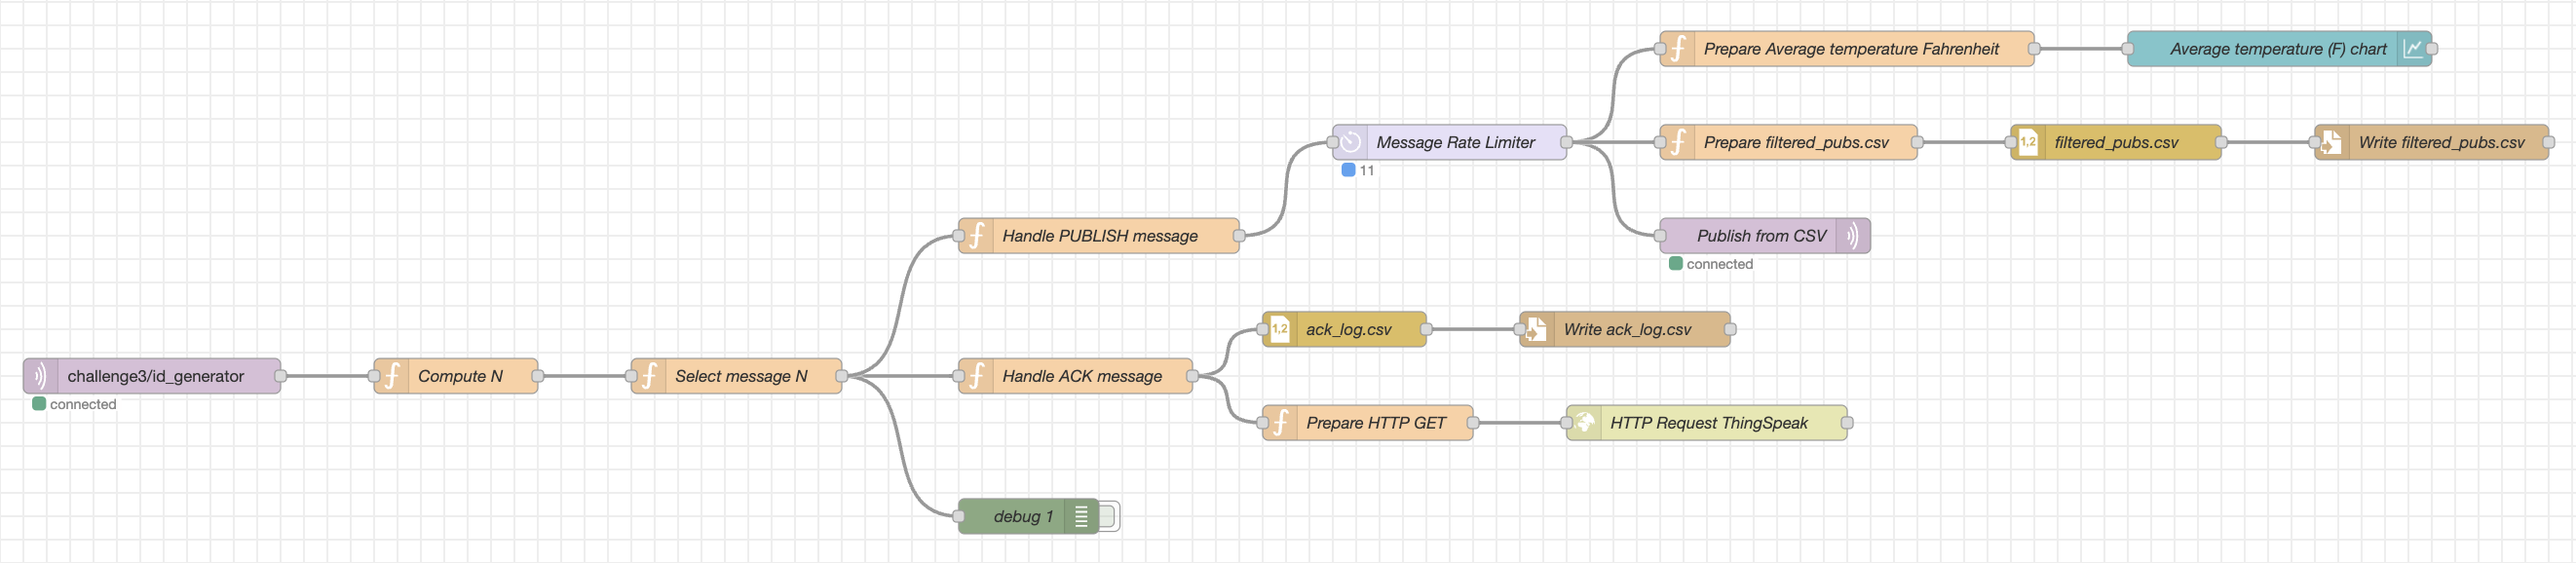
\includegraphics[width=\linewidth, height=0.5\textheight, keepaspectratio]{mqtt_subscriber_branch.png}
    \caption{MQTT Subscriber branch of the flow}
\end{figure}

\subsection{challenge3/id\_generator}
The first node is an mqtt in node, that is subscribed to the topic "challenge3/id\_generator" to the local MQTT broker on port 1884. This node receives messages sent to the local broker by the publisher in the first branch of the flow and processes them with the following nodes.

\subsection{Compute N}
This node is a function node that performs two main tasks:
\begin{itemize}
\item It increases by 1 the value of a context variable, called \verb|processed_messages|, that counts the number of messages processed up to a certain moment. The function node also checks if the value is greater than 80, in which case, the node discards the message.
\item The second task is performed only if the message needs to be processed: the node computes the value of N as N = id \% 7711, which will be needed to select the correct MQTT message from the CSV.
\end{itemize}

The code of the function node is reported here.
\begin{minted}{javascript}
var processedMessages = context.get("processed_messages") || 0;
processedMessages ++;
context.set("processed_messages", processedMessages);
if (processedMessages > 80) {
    return null;
}
var id = msg.payload["id"];
var N = id % 7711;
console.log(N);
// save id and N
msg.id = id;
msg.N = N;
return msg;
\end{minted}

\subsection{Select message N}
This node uses the value of N previously computed and extracts the correct row from the CSV file "challenge3.csv". If N is 0, the messages is discarded, since entries start from N=1, otherwise a row will be extracted. The function node reads the CSV from the flow variable \verb|csv_challenge3| and then filters the row with field "No." equal to N. The extracted message will be managed by the following two functions nodes, but at most one of them will actually use it to send a new message.

The code of the function node is reported here.
\begin{minted}{javascript}
if (msg.N === 0) {
  return null;
}
let rows = flow.get("csv_challenge3");
if (!rows) {
  console.log("NULL ROWS ")
  return null;
}
let target = rows.find(r =>
  parseInt(r["No."], 10) === msg.N
);
msg.payload = target;
return msg;
\end{minted}

\subsection{Handle PUBLISH message}
This node is a function node, it receives a message corresponding to the selected message from the CSV file "challenge3.csv", checks if it is a PUBLISH message and, if it is, prepares the new MQTT messages to publish. In order to prepare the messages to be published, we need to extract topics, extract payloads and map them together. 

\subsubsection{Topics}
The topics are contained in the "Info" field of the message and we can extract them with a regex, since they are in the form "Publish Message [	\textit{topic }]".

\subsubsection{Payloads}
The payloads, instead, are contained in the "Payload" field of the message. They are contained in curly braces and are similar to a JSON array, but without square brackets. 
We extract them by adding the missing square brackets and parsing them as a JSON array. There are some messages in which the payload is malformed and cannot be parsed as previously explained. We analyzed all PUBLISH messages with a Python script and found out that there are 3 messages with malformed payload and all of them have a certain number of well-formed messages, formed by a last message malformed message, which is truncated.\\
Since we don't want to waste the correct information contained in the "Payload" field, we use a regex to extract the payloads one at a time from opening curly brace to the corresponding closing one and we parse the text contained between curly braces as a JSON object. We discard the last, malformed, payload.\\
The Python script and the results of the run are reported here.

\begin{python}
import pandas as pd
import json 

df = pd.read_csv("challenge3.csv")

# filter MQTT PUBLISH messages 
publish_df = df[df['Info'].str.contains('Publish Message', na=False)]

# filter ACK messages 
ack_df = df[df['Info'].str.contains("Connect Ack", na=False)] + df[df['Info'].str.contains("Publish Ack", na=False)] + df[df['Info'].str.contains("Subscribe Ack", na=False)]

invalid_rows_publish = []
invalid_rows_ack = []

# find invalid PUBLISH messages
for idx, raw_payload in zip(publish_df.index, publish_df['Payload']):
    payload_str = raw_payload if isinstance(raw_payload, str) else ''
    if not payload_str.strip():
        continue
    try:
        json.loads(f'[{payload_str}]')
    except json.JSONDecodeError as e:
        print(f"Errow No. {idx+1}: {e}")
        invalid_rows_publish.append(idx + 1)
print("No. invalid rows publish:", invalid_rows_publish)

# find invalid ACK messages
for idx, raw_payload in zip(ack_df.index, ack_df['Payload']):
    payload_str = raw_payload if isinstance(raw_payload, str) else ''
    if not payload_str.strip():
        continue
    try:
        json.loads(f'[{payload_str}]')
    except json.JSONDecodeError as e:
        print(f"Errow No. {idx+1}: {e}")
        invalid_rows_ack.append(idx + 1)
print("No. invalid rows ack:", invalid_rows_ack)
\end{python}

\begin{figure}[H]
    \centering
    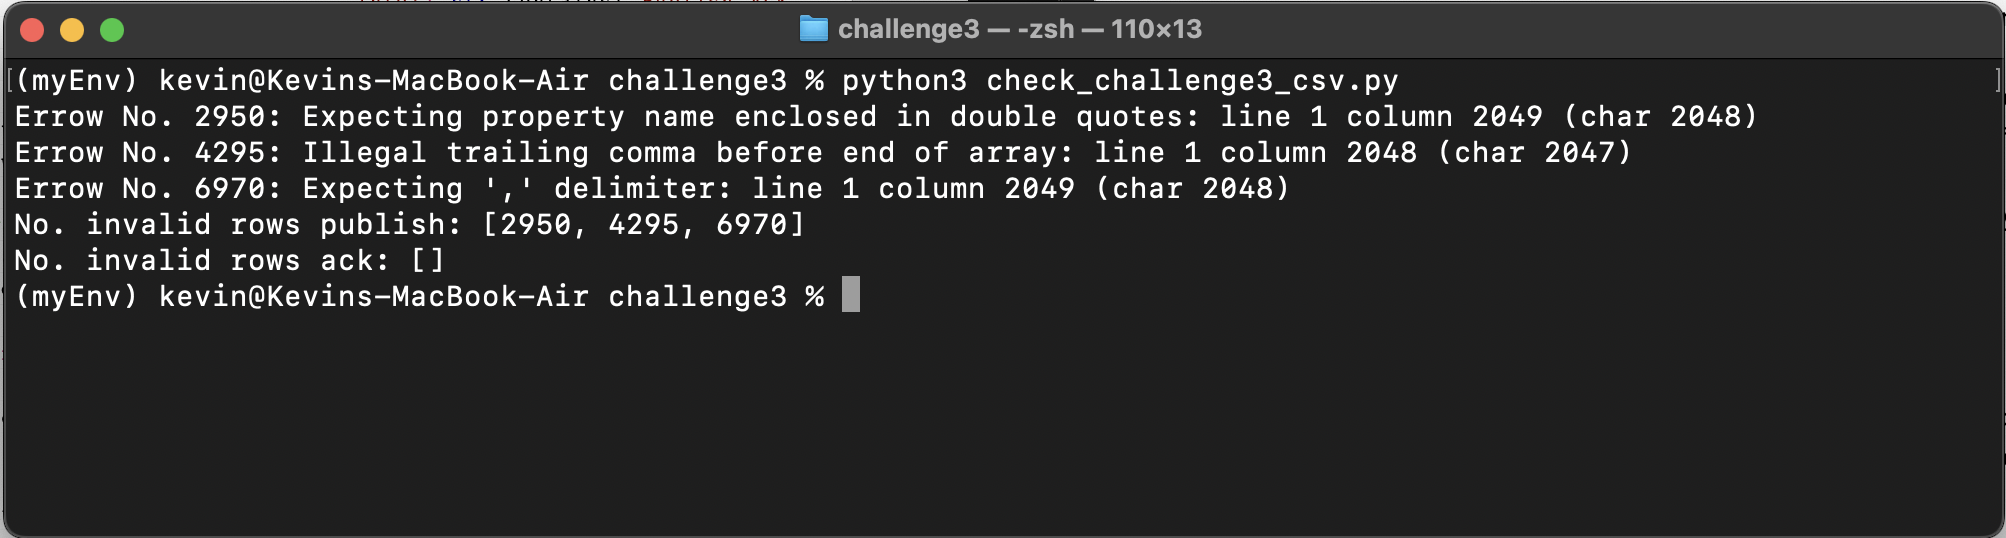
\includegraphics[width=\linewidth, height=0.5\textheight, keepaspectratio]{malformed_script_run.png}
    \caption{Python script malformed messages run}
\end{figure}

\subsubsection{Complete messages}
Finally, we need to combine topics and payloads, we do that by using the map operation. If the number of topics is greater than the number of payloads, we assign an empty payload to the topics without a payload. Beyond topic and payload, the produced messages will have the current timestamp and the id, which was saved in the message from the Compute N function node.
The produced MQTT message will have the following form:
\begin{verbatim}
'{
    "timestamp":"CURRENT_TIMESTAMP",
    "id":"SUB_ID",
    "topic":"MQTT_PUBLISH_TOPIC",
    "payload":"MQTT_PUBLISH_PAYLOAD"
}'
\end{verbatim}
In order to have the timestamp and id quoted, we convert them to strings inside the function node. 

The code of the function node is reported here.
\begin{minted}{javascript}
if (msg.payload["Protocol"] === "MQTT" && 
	msg.payload["Info"].includes("Publish Message")) {
    // save info in a variable
    let info = msg.payload["Info"];
    // save messages payloads in a variable
    let messagesPayloads = msg.payload["Payload"] ?? "";
    // extract topics
    let topicMatches = [...info.matchAll(/Publish Message \[([^\]]+)\]/g)];
    let topics = topicMatches.map(m => m[1]);
    // extract payloads
    let jsonArray;
    if (messagesPayloads.trim() === "") {
        jsonArray = [];
    } else {
        try {
            jsonArray = JSON.parse("[" + messagesPayloads + "]");
        } catch (e) {
            // extract well formed messages

            const objs = [];
            const objRegex = /\{[^}]*\}/g;
            let m;
            while ((m = objRegex.exec(messagesPayloads)) !== null) {
                try {
                objs.push(JSON.parse(m));
                } catch (_) {
                    // skip malformed object
                }
            }
            jsonArray = objs;
        }
    }
    // create messages 
    var currTimestamp = Math.floor(Date.now() / 1000);
    let messages = topics.map((topic, index) => {
        return {
            topic: topic, 
            payload: {
                timestamp: currTimestamp.toString(),
                id: msg.id.toString(),
                topic: topic,
                payload: jsonArray[index] ?? {}
            }
        };
    });
    return [messages];
}
return null;
\end{minted}

\subsection{Message Rate Limiter}
Among all extracted messages, we need to publish up to 4 messages per minute. We do that thanks to a delay node, that is set to work with action "Rate Limit" and limit the rate to 4 messages per minute, queueing intermediate messages.  

\subsection{Publish from CSV}
This node is a mqtt out node that publishes messages that manage to go through the Message Rate Limiter. They are published to the local broker, on a dynamic topic, that was extracted from the CSV file and is saved in the message itself.\\
We show the correct functioning by subscribing to a topic from a terminal and showing the message arriving to the subscriber.

\begin{figure}[H]
    \centering
    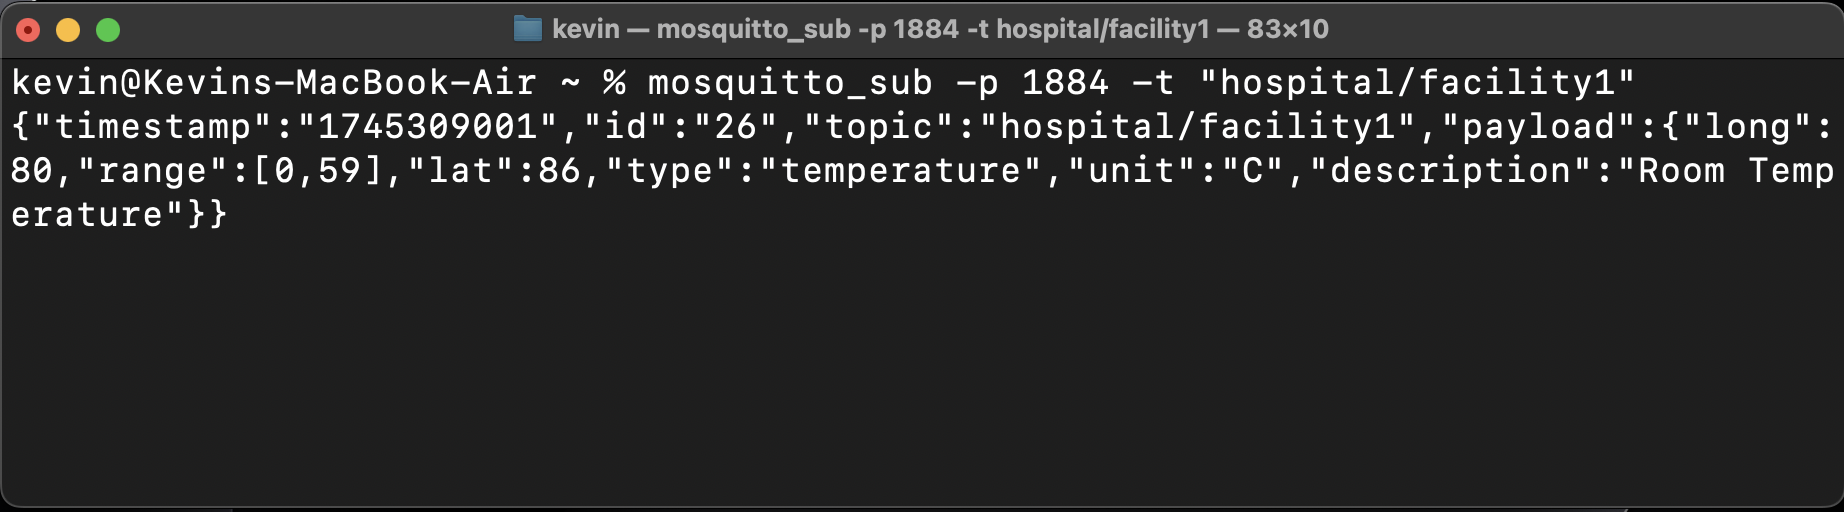
\includegraphics[width=\linewidth, height=0.5\textheight, keepaspectratio]{mqtt_subscriber.png}
    \caption{MQTT client subscribed to topic "hospital/facility1"}
\end{figure}

\subsection{Prepare Average temperature Fahrenheit}
This node is a function node that receives messages that went through the rate limiter and were published. The function checks if the value contained in the payload of the message is a temperature in Fahrenheit and, if it is, computes the average temperature starting from the range contained the in the payload. The prepared message will be used to plot the average temperature in Fahrenheit.

The code of the function node is reported here.
\begin{minted}{javascript}
if (msg.payload.payload.type === "temperature" 
	&& msg.payload.payload.unit === "F") {
    let minTemp = msg.payload.payload.range[0];    
    let maxTemp = msg.payload.payload.range[1];
    let avgTemp = (minTemp + maxTemp)/2;
    msg.topic = "TempF";
    msg.payload = avgTemp;
    return msg;
}
return null
\end{minted}

\subsection{Average temperature (F) chart}
This node is a chart node and is used to plot in Node-RED the average temperature in Fahrenheit of the published messages.\\
An example of produced chart is reported here.

\begin{figure}[H]
    \centering
    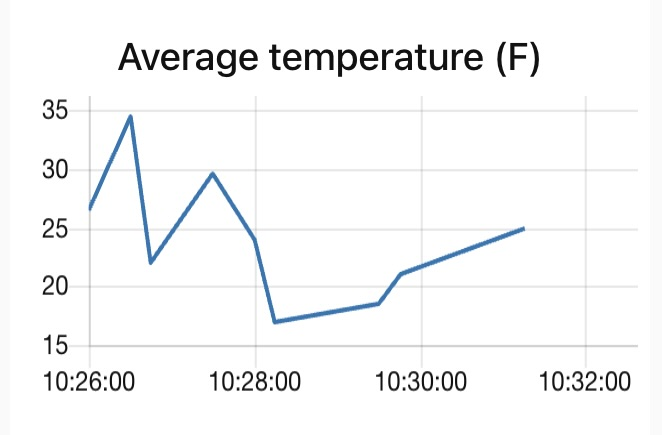
\includegraphics[width=0.5\linewidth, height=0.5\textheight, keepaspectratio]{avg_temp_chart_node_red.jpeg}
    \caption{Average Fahrenheit temperature chart in Node-RED}
\end{figure}

\subsection{Prepare filtered\_pubs.csv}
This function node takes all PUBLISH messages that were published and filters the same ones as the other function node, i.e. all the ones containing a temperature in Fahrenheit. The function increases by one the counter for the number of rows in the CSV file filtered\_pubs.csv, contained in the context variable \verb|row_count_filtered_pubs|. Moreover, the function produces the new row of the CSV using the data contained in the payload of the message and the value of the row counter. The payload must be a JSON object with fields matching the ones of the CSV, in order to work seamlessly with the csv node.

The code of the function node is reported here.
\begin{minted}{javascript}
if (msg.payload.payload.type === "temperature" 
	&& msg.payload.payload.unit === "F") {
    var counter = context.get("row_ count_filtered_pubs") || 0;
    counter++;
    context.set("row_count_filtered_pubs", counter);
    let data = msg.payload.payload;
    let meanValue = (data.range[0] + data.range[1]) / 2;
    let long = data.long;
    let lat = data.lat;
    let type = data.type;
    let unit = data.unit;
    let desc = data.description;
    msg.payload = {
        "No." : counter,
        "LONG": long,
        "LAT": lat,
        "MEAN_VALUE": meanValue,
        "TYPE": type,
        "UNIT": unit,
        "DESCRIPTION": desc
    }
    return msg;
}
return null;
\end{minted}

\subsection{filtered\_pubs.csv}
This node is a csv node and is used in the "Object to CSV" way to save the JSON object contained in the payload to a row of the CSV. At first, the node produces the header: No.,LONG, LAT, MEAN\_VALUE, TYPE, UNIT, DESCRIPTION. Then it produces the following lines based on the JSON object it receives, which has the same fields as the CSV.

\subsection{Write filtered\_pubs.csv}
This node is a write file node as is used to write the actual CSV file filtered\_pubs.csv, which is saved to a location on the disk specified in the path inside the node.

\subsection{Handle ACK message}
This node is a function node that is used to handle ACK messages retrieved from the challenge3.csv file. The function checks if the message is an MQTT ACK message, looking at the "Info" field: if it contains the word "Ack", it is an ACK message. The function increases a row counter for the CSV file ack\_log.csv, contained the context variable \verb|row_count_ack_log| and prepares the JSON object to be written in the CSV. The produced messages will have in the payload all fields of the CSV file ack\_log.csv: the incremental row counter in "No.", the current timestamp, the id of the original message and the message type, which the function finds in the "Info" field, together with the "Ack" keyword.

The code of the function node is reported here.
\begin{minted}{javascript}
if (msg.payload["Protocol"] === "MQTT" 
	&& msg.payload["Info"].includes("Ack")) {
    var counter = context.get("row_count_ack_log") || 0;
    counter++;
    context.set("row_count_ack_log", counter);
    var currTimestamp = Math.floor(Date.now() / 1000);
    let idMatch = msg.id;
    var type = "";
    if (msg.payload["Info"].includes("Connect Ack")) {
        type = "Connect Ack";
    } else if (msg.payload["Info"].includes("Publish Ack")){
        type = "Publish Ack";
    } else if (msg.payload["Info"].includes("Subscribe Ack")) {
        type = "Subscribe Ack";
    }
    msg.payload = {
        "No.": counter,
        "TIMESTAMP": currTimestamp,
        "SUB_ID": idMatch,
        "MSG_TYPE": type
    }
    return msg;
}
return null;
\end{minted}

\subsection{ack\_log.csv}
This node is a csv node and is used in the "Object to CSV" way to save the JSON object contained in the payload to a row of the CSV ack\_log.csv. The csv node produces a header No., TIMESTAMP, SUB\_ID, MSG\_TYPE and all the rows of the CSV, matching the fields of the CSV with the ones of the message payload.

\subsection{Write ack\_log.csv}
This node is a write file node as is used to write the actual CSV file ack\_log.csv, which is saved to a location on the disk specified in the path inside the node.

\subsection{Prepare HTTP GET}
This node is a function node that prepares the HTTP message to send to the ThingSpeak channel. It sets the method to GET and the URL to the one exposed by the API, passing the API KEY and the value of the global ack counter, contained in the message payload and computed in the Handle ACK message function node.

The code of the function node is reported here.
\begin{minted}{javascript}
var API_KEY="SECRET_API_KEY"
var globalCounter = msg.payload["No."]
msg.method = "GET";
msg.url = "https://api.thingspeak.com/update?api_key="+
	API_KEY+"&field1="+globalCounter

return msg;
\end{minted}

\subsection{HTTP Request ThingSpeak}
This node is an http request node that sends the HTTP request, using the method and URL set in the message.\\
An example of produced chart is reported here.
\begin{figure}[H]
    \centering
    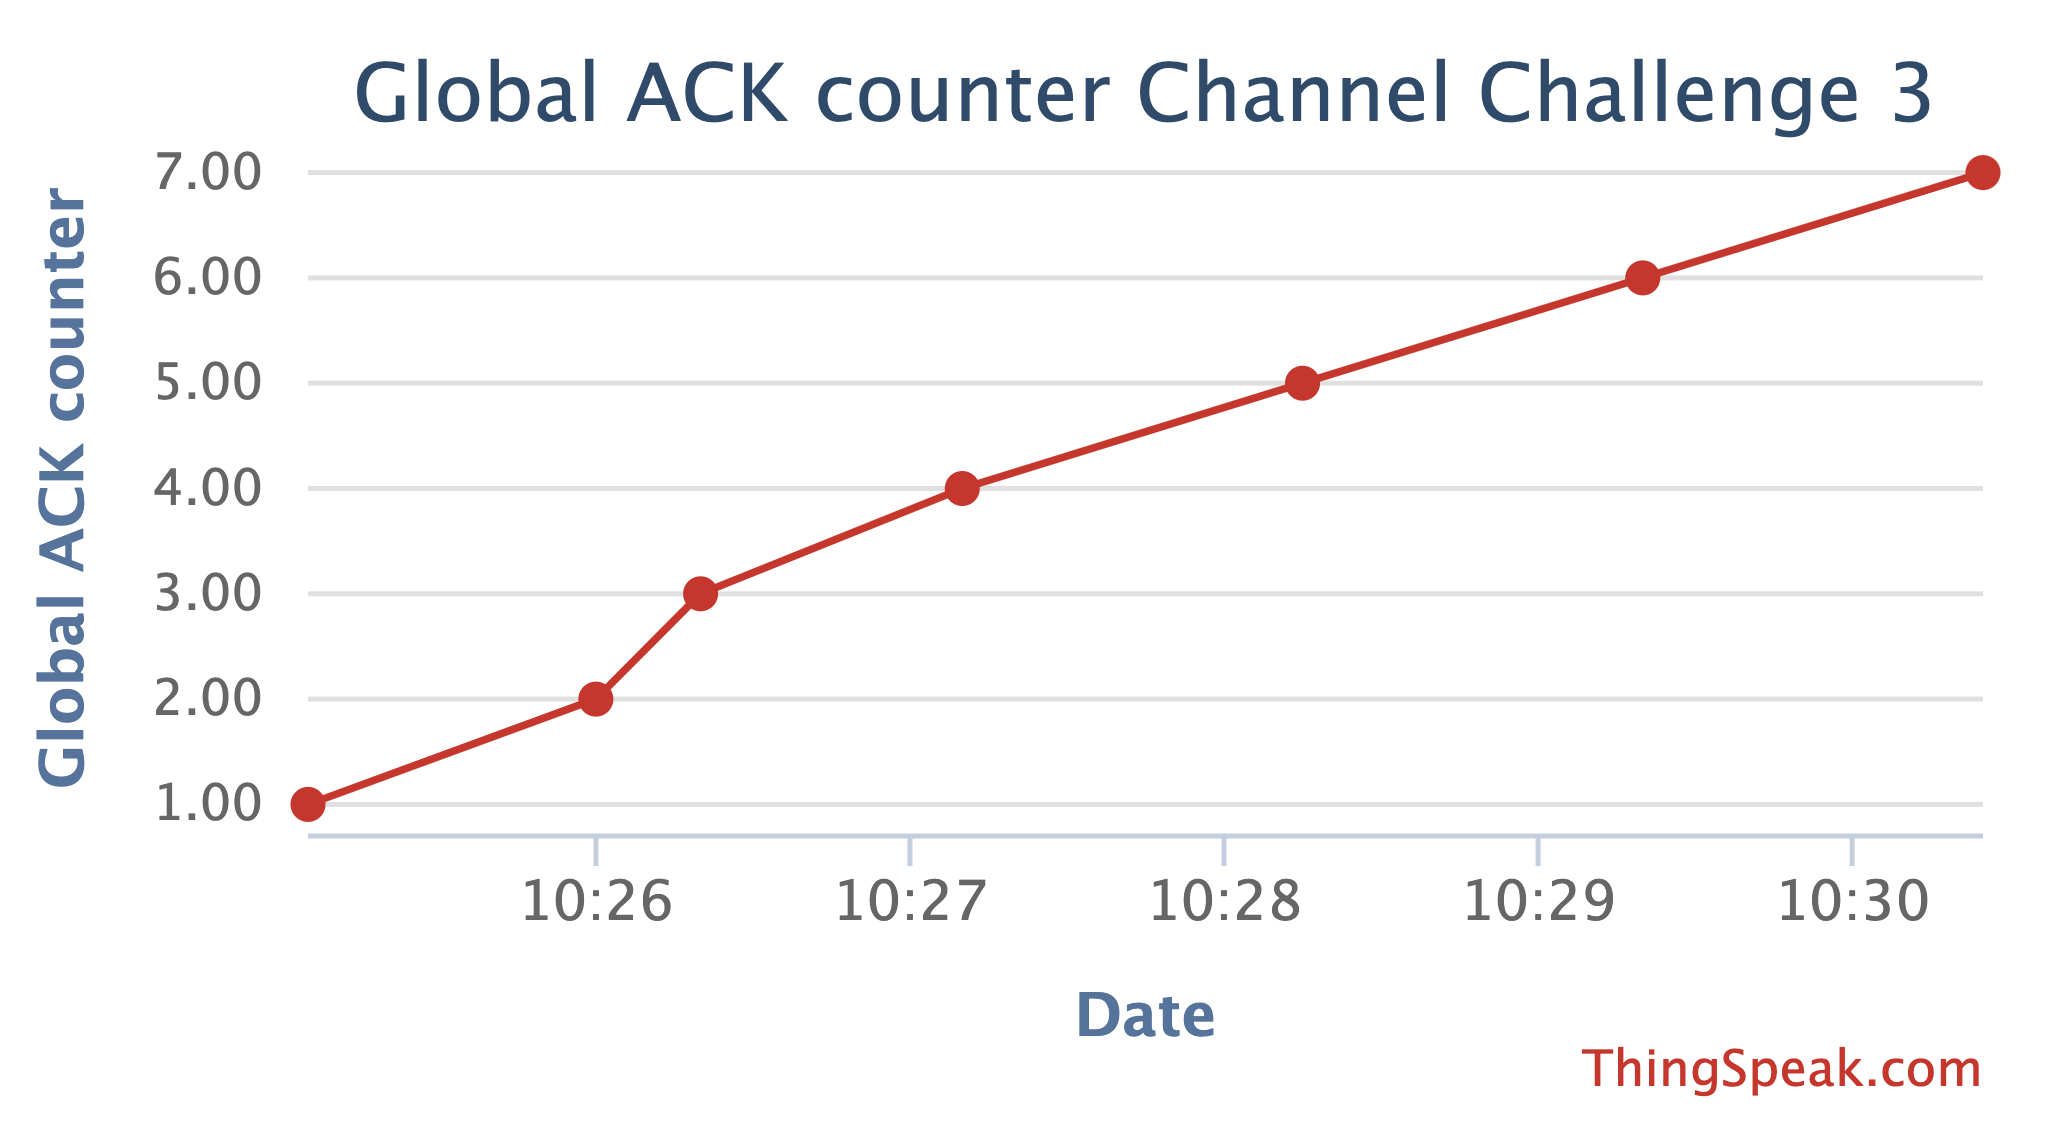
\includegraphics[width=0.5\linewidth, height=0.5\textheight, keepaspectratio]{global_ack_counter_chart_thingspeak.png}
    \caption{Global ACK counter chart in ThingSpeak}
\end{figure}



